\chapter{Task}
Uno scenario di machine learning predittivo è quello in cui, dato un set di dati etichettati, viene chiesto a un algoritmo di apprendimento di costruire un modello in grado di fare previsioni su “alcune proprietà” di nuovi esempi (mai visti in precedenza).

A seconda del tipo di etichette associate ai dati e di quale “\textbf{proprietà}” l’algoritmo deve prevedere, possiamo distinguere tra i seguenti compiti: \textbf{classificazione}, \textbf{scoring} e \textbf{ranking}, \textbf{stima della probabilità} e \textbf{regressione}.

\section{Classificazione}
Un \textbf{classificatore} fa una mappatura di questo tipo:
\begin{equation}
\begin{split}
    \hat{c} : X \rightarrow C \\
    C={C_1,C_2,\dots,C_K}
\end{split}
\end{equation}
$X$ è lo \textbf{spazio degli esempi} e $C$ è lo \textbf{spazio delle classi}.
Il \textbf{cappello} sopra $C$ indica che è un'approssimazione del concetto reale.
Costruire un classificatore implica costruire la funzione $\hat{c}$ in modo tale che corrisponda a $c$ il più fedelmente possibile (e non solo sul training set, ma idealmente sull'intero spazio delle istanze $X$).

Un esempio è la coppia:
\begin{equation}
    (x,c(x))\in X \times C
\end{equation}
dove $x$ è un' \textbf{istanza} e $c(x)$ è la classe reale a cui appartiene l'istanza.

\paragraph{Classificazione binaria.} E' il caso particolare in cui l'insieme delle classi $C$ contiene solo le classi 0 e 1 (o true e false).
Dalla classificazione binaria si può passare a quella multiclasse senza cambiare algoritmo.
\begin{figure}
    \centering
    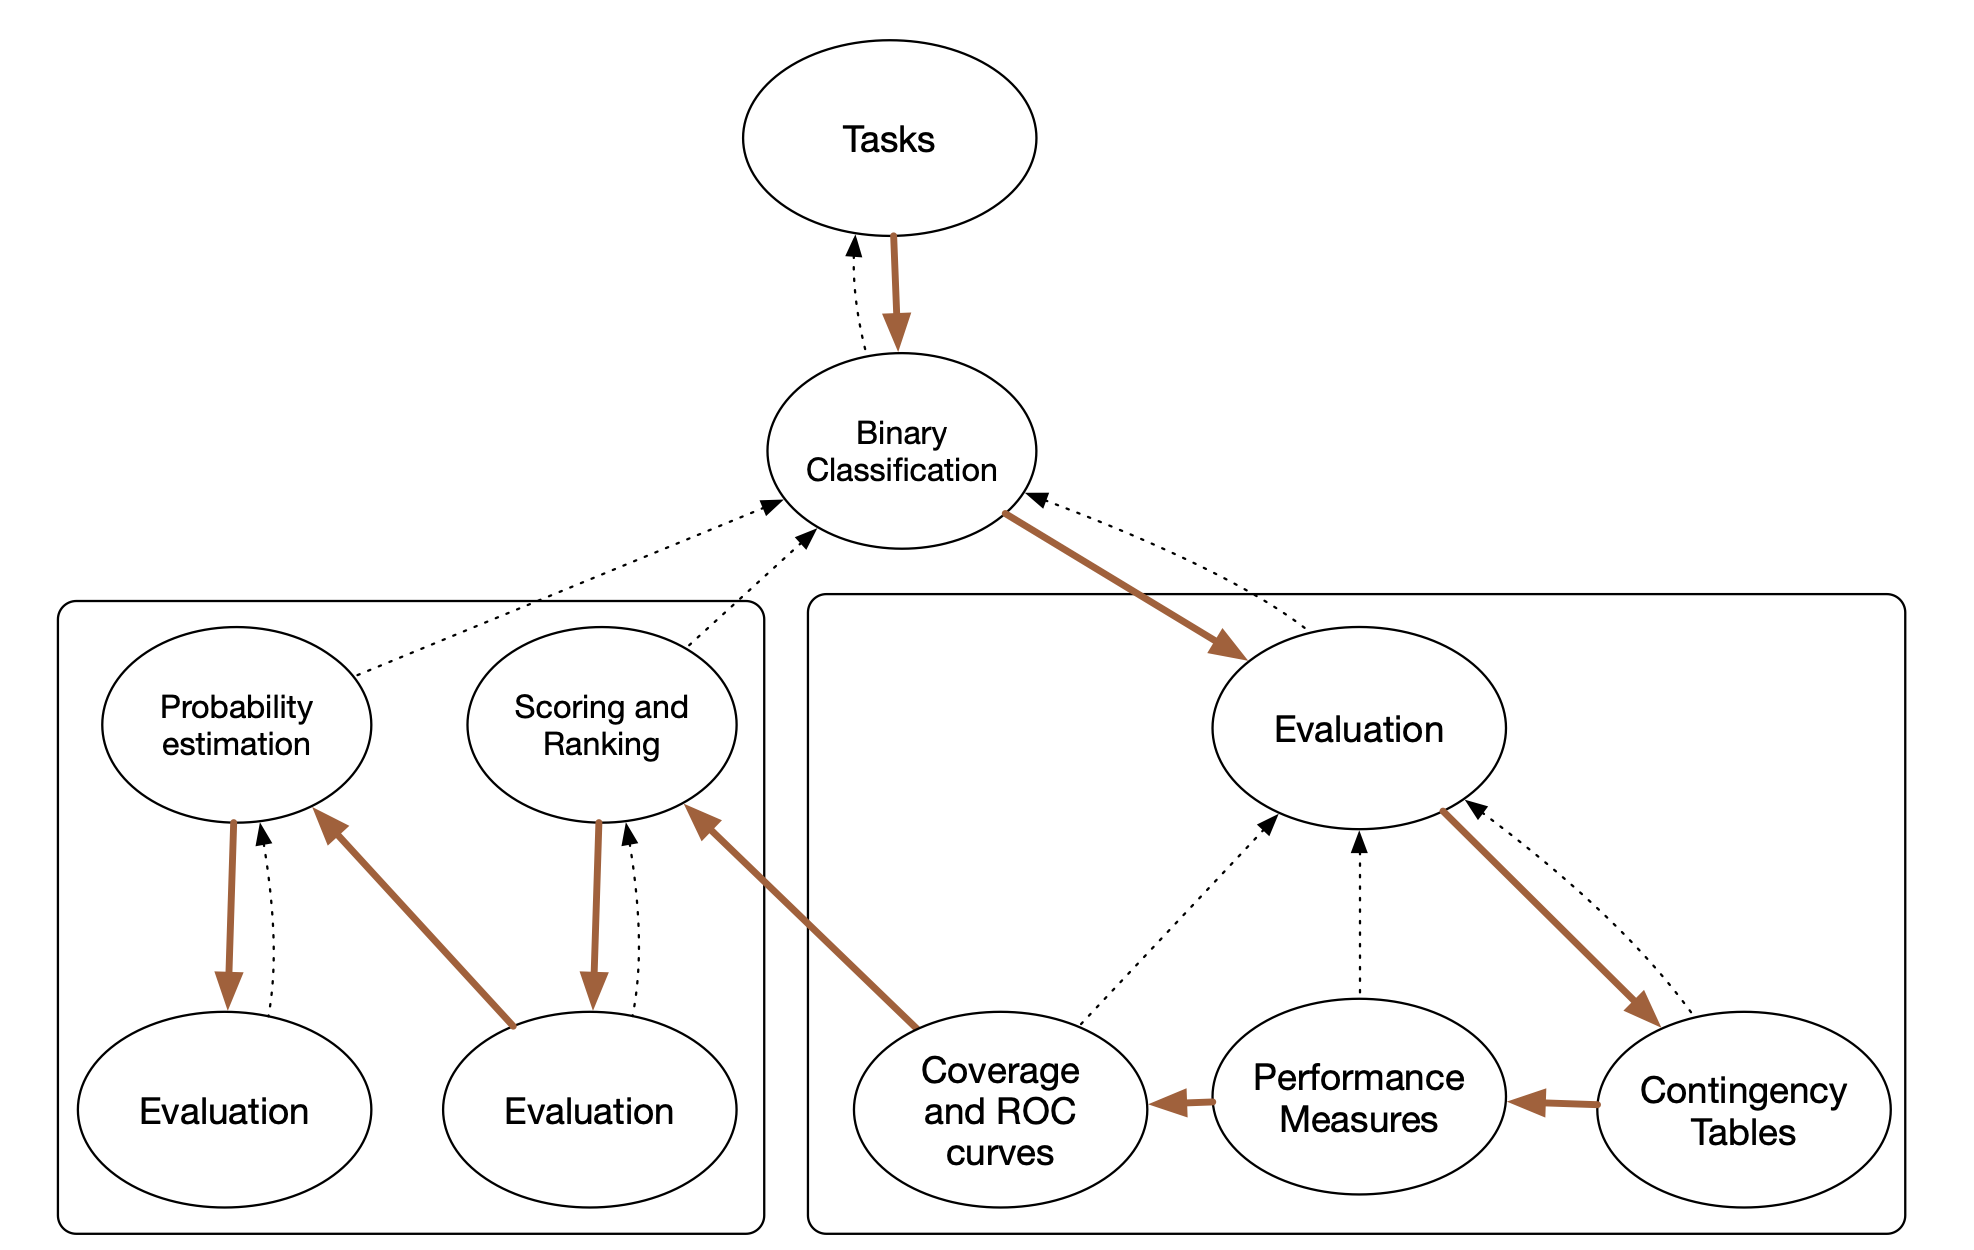
\includegraphics[scale=0.2]{images/binClassifier.png}
    \caption{Binary classification topics}
    \label{fig:enter-label}
\end{figure}

\newpage

\paragraph{Valutazione} Introduciamo gli \textbf{alberi di decisione}. L'esempio è il solito sull'etichettatura dell'email. L'idea è che ogni \textbf{nodo} corrisponde ad una \textbf{feature} ('viagra' e 'lottery' in questo caso) e se quella feature è presente seguo un ramo, altrimenti seguo l'altro. Arrivato al fondo ottengo l'etichetta.

Gli \textbf{alberi di feature} sono analoghi ma nelle foglie ho il numero degli esempi del training set che sono finiti in quella foglia, suddivisi nelle varie classi.

\begin{figure}[!h]
    \centering
    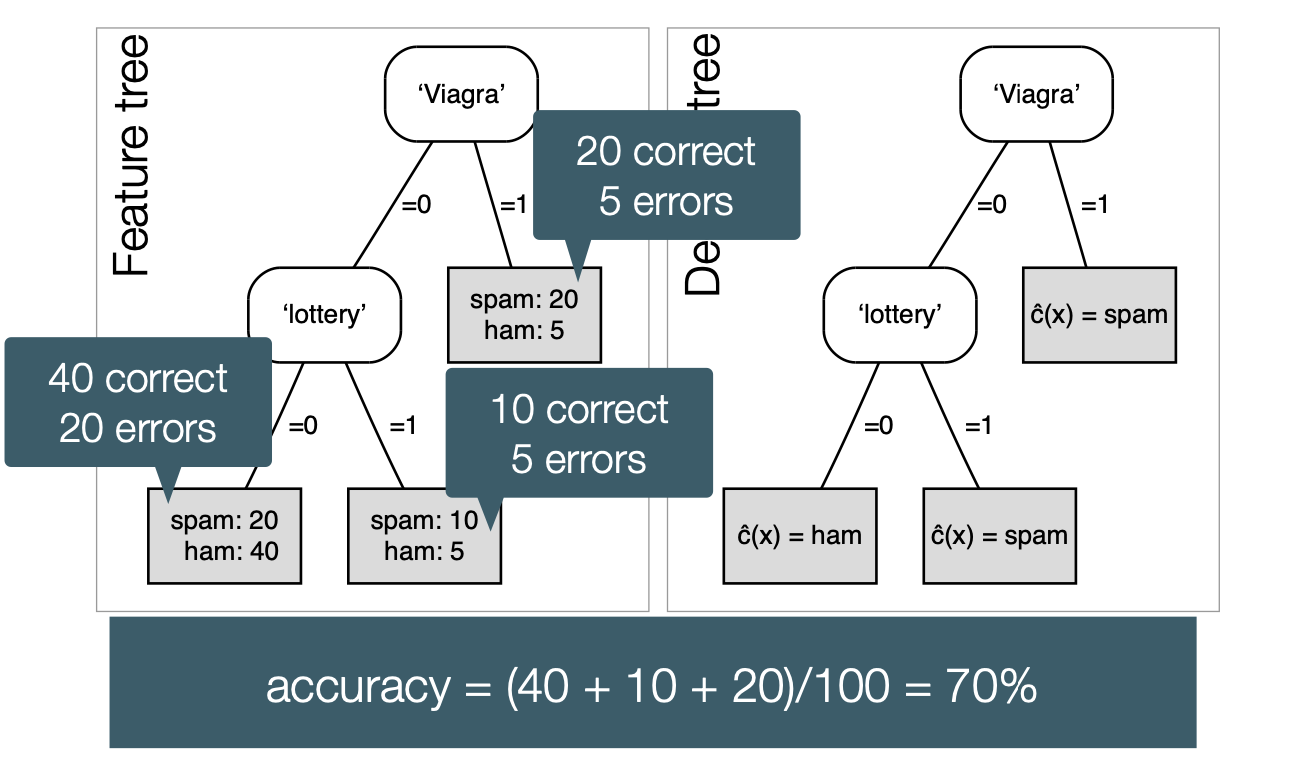
\includegraphics[scale=0.6]{images/featureTree.png}
    \label{fig:enter-label}
\end{figure}
Guardando i numeri e le etichette si calcola l'\textbf{accuratezza}, che è una delle misure che si usano per valutare il modello. Non è l'unica però, infatti nasconde molte informazioni. 

Nella \textbf{tavola di contingenza} (nel caso binario una tavola $2x2$), le colonne corrispondono a ciò che abbiamo predetto e le righe alle etichette che ci sono state date. Nelle interesezioni ci sono gli esempi che sono stati predetti in un certo modo e che hanno una certa etichetta.
\begin{figure}[!h]
    \centering
    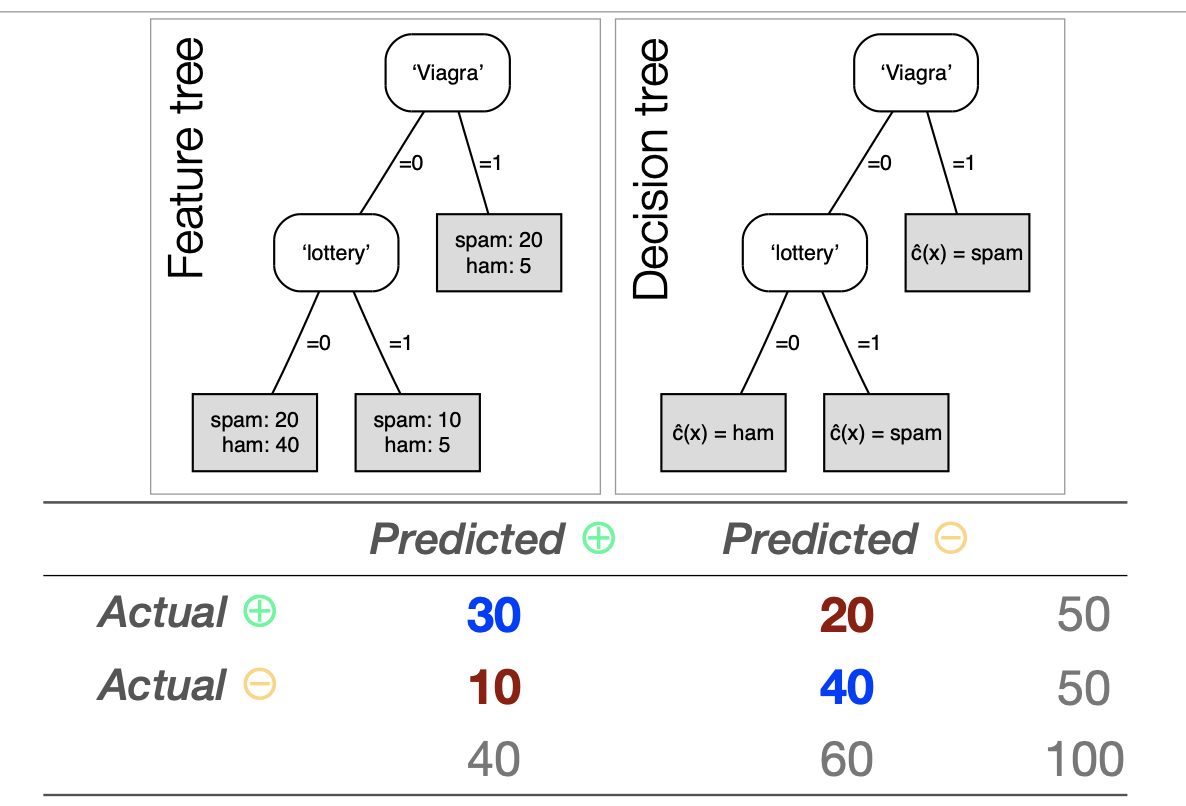
\includegraphics[scale=0.6]{images/contTable.png}
    \caption{Tavola di contingenza}
    \label{fig:enter-label}
\end{figure}

\newpage

Introduciamo un po' di notazione:
\begin{itemize}
    \item \textbf{TP}, \textbf{true positive}, quelli che ho predetto essere positivi e che sono effettivamente positivi;
    \item \textbf{FP}, \textbf{false positive}, quelli che ho predetto essere positivi e che sono però negativi;
    \item \textbf{FN}, \textbf{false negative}, quelli che ho predetto essere negativi e che sono però positivi;
    \item \textbf{TN}, \textbf{true negative}, quelli che ho predetto essere negativi e che sono effettivamente negativi;
\end{itemize}

\begin{equation}
\begin{split}
    TP+FN=POSITIVE  \\
    FP+TN=NEGATIVE
\end{split}
\end{equation}

\begin{figure}[!h]
    \centering
    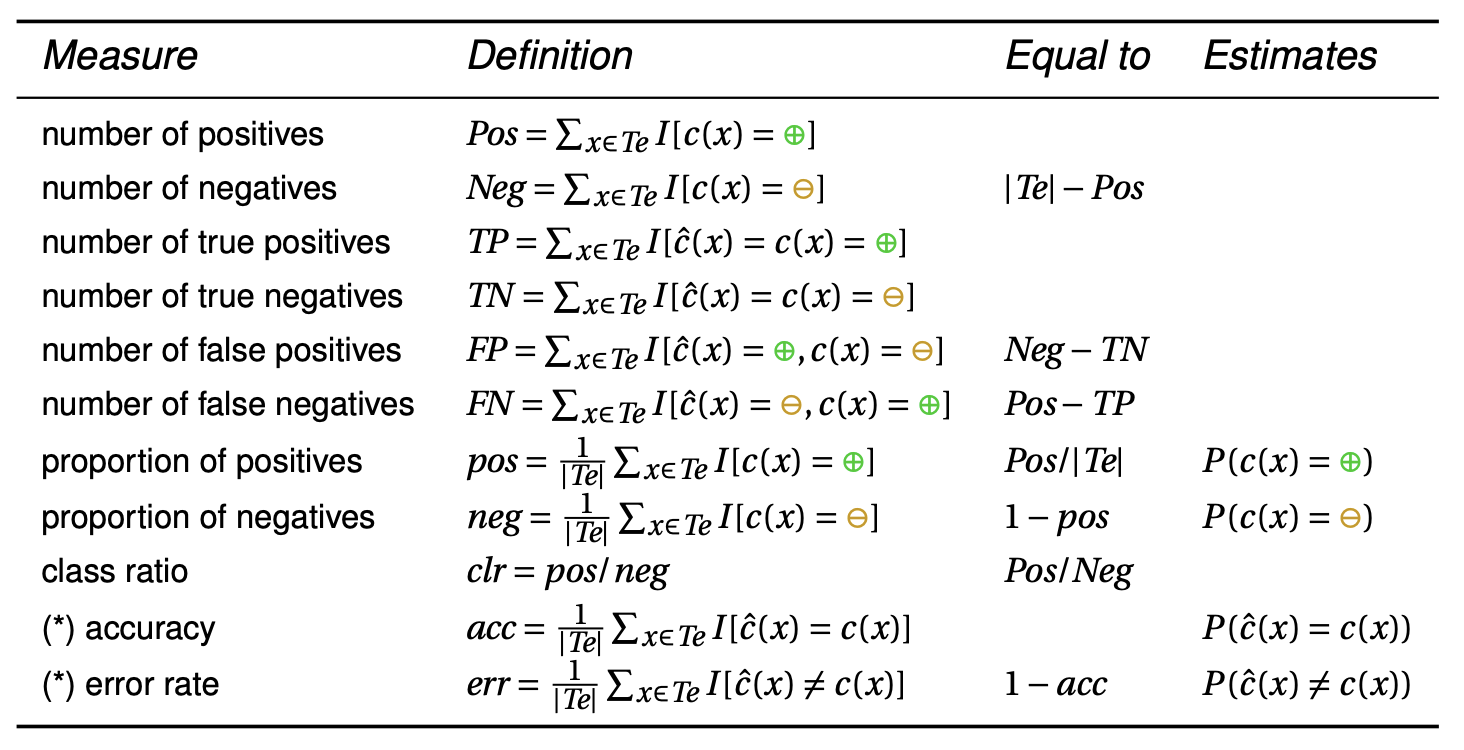
\includegraphics[scale=0.7]{images/measures.png}
    \caption{Misurazioni di performance}
    \label{fig:enter-label}
\end{figure}

\newpage

\paragraph{Coverage plot.} Il \textbf{coverage plot} è un modo per mettere in un grafico le informazioni che ci sono nella tavola di contingenza. I FP sono sull'asse delle x, i TP sull'asse delle y e mettiamo un punto sul grafico in corrispondenza del punto considerato della tavola di contingenza.
\begin{figure}[!h]
    \centering
    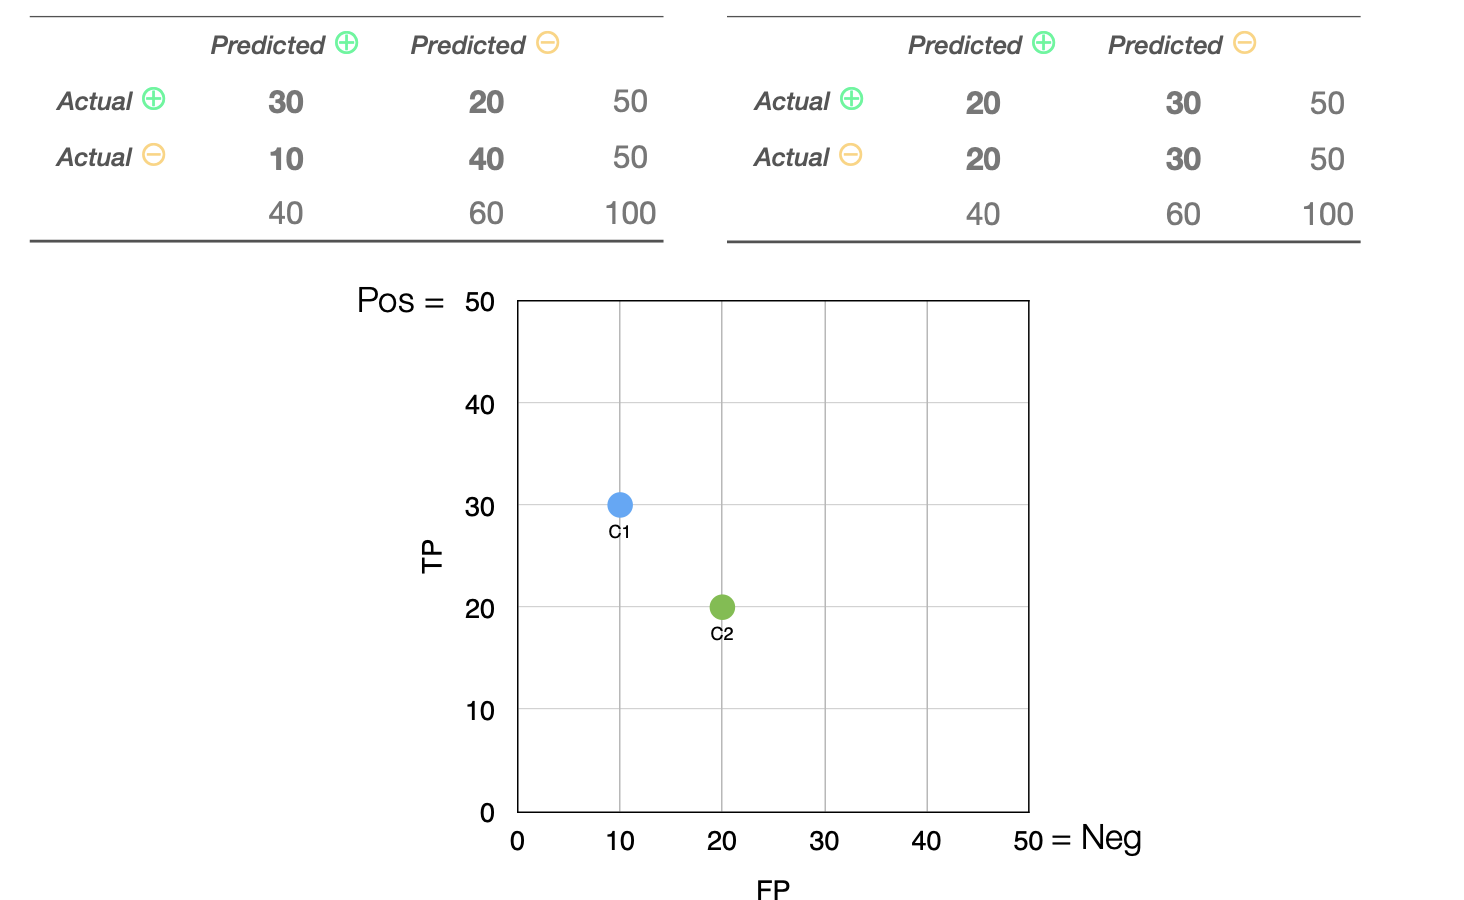
\includegraphics[scale=0.5]{images/covPlot.png}
    \label{fig:enter-label}
\end{figure}

Sembrerebbero mancare gli esempi che non sono stati predetti come positivi, ma questo non è un problema. Possiamo infatti calcolare i FN come $POS-TP$ e TN come $NEG-FP$. Quindi in verità nel grafico è rapprensentata tutta l'informazione della tavola di contingenza.

\textbf{Per cosa lo utilizziamo?} Lo utilizziamo capire quale classificatore è migliore. In questo caso sembra essere $c_1$ poichè ha un numeri di TP più alto ma anche un numero di TN più alto. 

Nel grafico ci sono 2 zone chiamate \textbf{ROC heaven} e \textbf{ROC hell}. \textbf{ROC heaven} è la zona del grafico che corrisponde a dove vorrei che fossero i miei classificatori (in alto a sinistra), al contrario \textbf{ROC hell} è una zona che descrive un classificatore che sbaglia sempre. In realtà però il punto peggiore è un altro poichè se un classificatore è nel ROC hell basta prendere il contrario delle etichette che fornisce. Il posto peggiore è la \textbf{diagonale principale}, li ci sono i classificatore che sostanzialmente tirano a caso.

Due classificatori sono uguali (cioè hanno la stessa accuratezza) se hanno la stessa distanza dall'angolo in alto a sinistra e si dice che sono su una \textbf{isometria di accuratezza}.

\begin{figure}
    \centering
    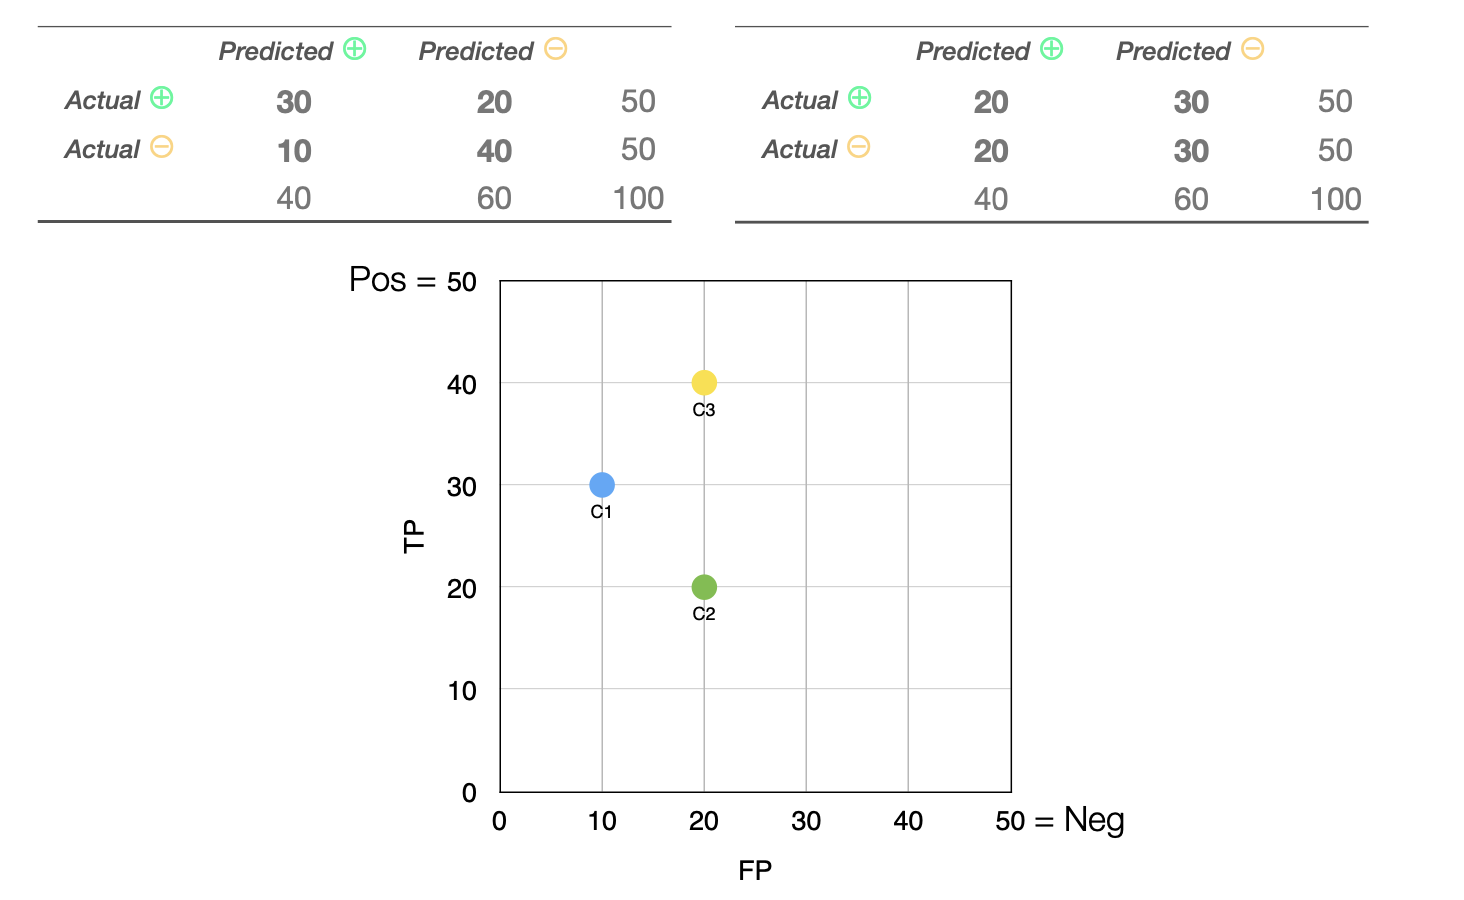
\includegraphics[scale=0.45]{images/accIso.png}
    \caption{Due classificatore sulla isometria di accuratezza}
    \label{fig:enter-label}
\end{figure}

\newpage

\paragraph{Proprietà del coverage plot.} Formalizziamo il concetto introdotto prima: i classificatori con la stessa \textbf{accuratezza} si trovano su una linea con \textbf{pendenza 1}.
L'accuratezza è data da
\begin{equation}
    ACC = \frac{TP+TN}{TOT}.
\end{equation}
Notiamo che se ci spostiamo a destra e in alto di uno:
\begin{equation}
\begin{split}
    ACC = \frac{(TP+1)+(TN-1)}{TOT} \\
    ACC = \frac{TP+TN}{TOT}.
\end{split}
\end{equation}

Tutti i classificatori con la stessa \textbf{average recall}, sono sulla stessa linea che è \textbf{parallela alla diagonale principale}. L'average recall è la media tra la positive recall e la negative recall che sono così definite:
\begin{equation}
\begin{split}
    POS\cdot REC=\frac{TP}{POS}   \\
    NEG\cdot REC=\frac{TN}{POS}   \\
    avg\cdot recall = \frac{(pos\cdot reg+neg\cdot rec)}{2}
\end{split}
\end{equation}

\begin{figure}[!h]
    \centering
    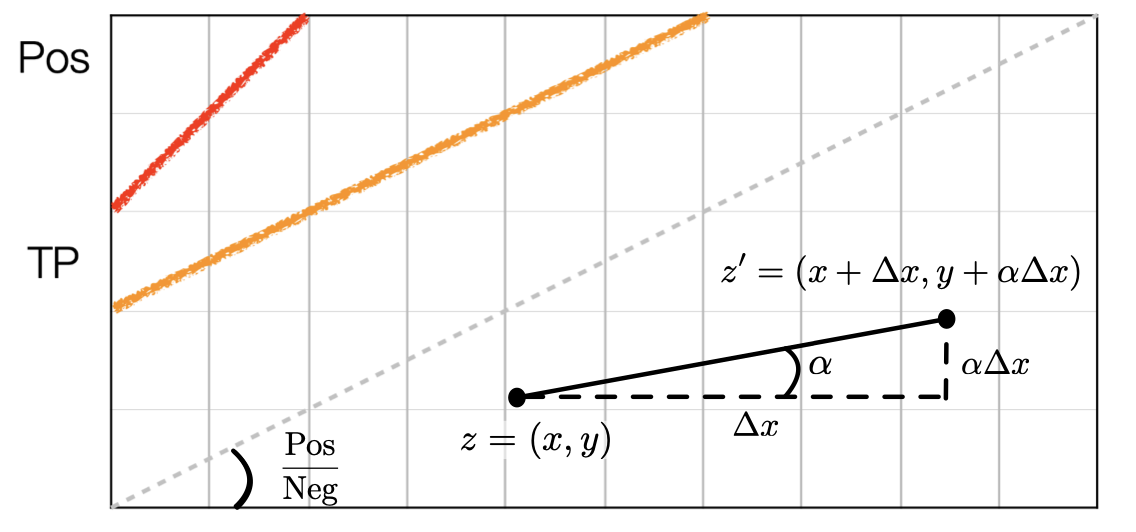
\includegraphics[scale=0.6]{images/avgRec.png}
    \label{fig:enter-label}
\end{figure}

Vogliamo calcolare la pendenza della retta su cui giacciono due esempi che hanno la stessa avg recall.
\begin{equation}
\begin{split}
    avgrec(z)=\left(\frac{y}{Pos}+\frac{Neg-x}{Neg} \right)/2 \\
    avgrec(z)=\left(\frac{y+\alpha \Delta x}{Pos}+\frac{Neg-x-\Delta x}{Neg} \right)/2 =\\
    avgrec(z)=\left(\frac{y}{Pos}+\alpha\frac{\Delta x}{Pos}+\frac{Neg-x}{Neg}-\frac{\Delta x}{Neg} \right)/2
\end{split}
\end{equation}
Quindi $z$ e $z^{'}$ hanno la stessa avg-rec \textbf{se e solo se} $\alpha\frac{Pos}{Neg}$.

\newpage

\paragraph{Roc Plots.} L'unica differenza con i coverage plot è che normalizziamo gli assi ad dividendo le y per Neg e le x per Pos. Il vantaggio è che possiamo confrontare classificatori che sono stati addestrati su dataset di dimensioni diverse.

Vediamo le differenza con il coverage plot.
\begin{figure}[!h]
    \centering
    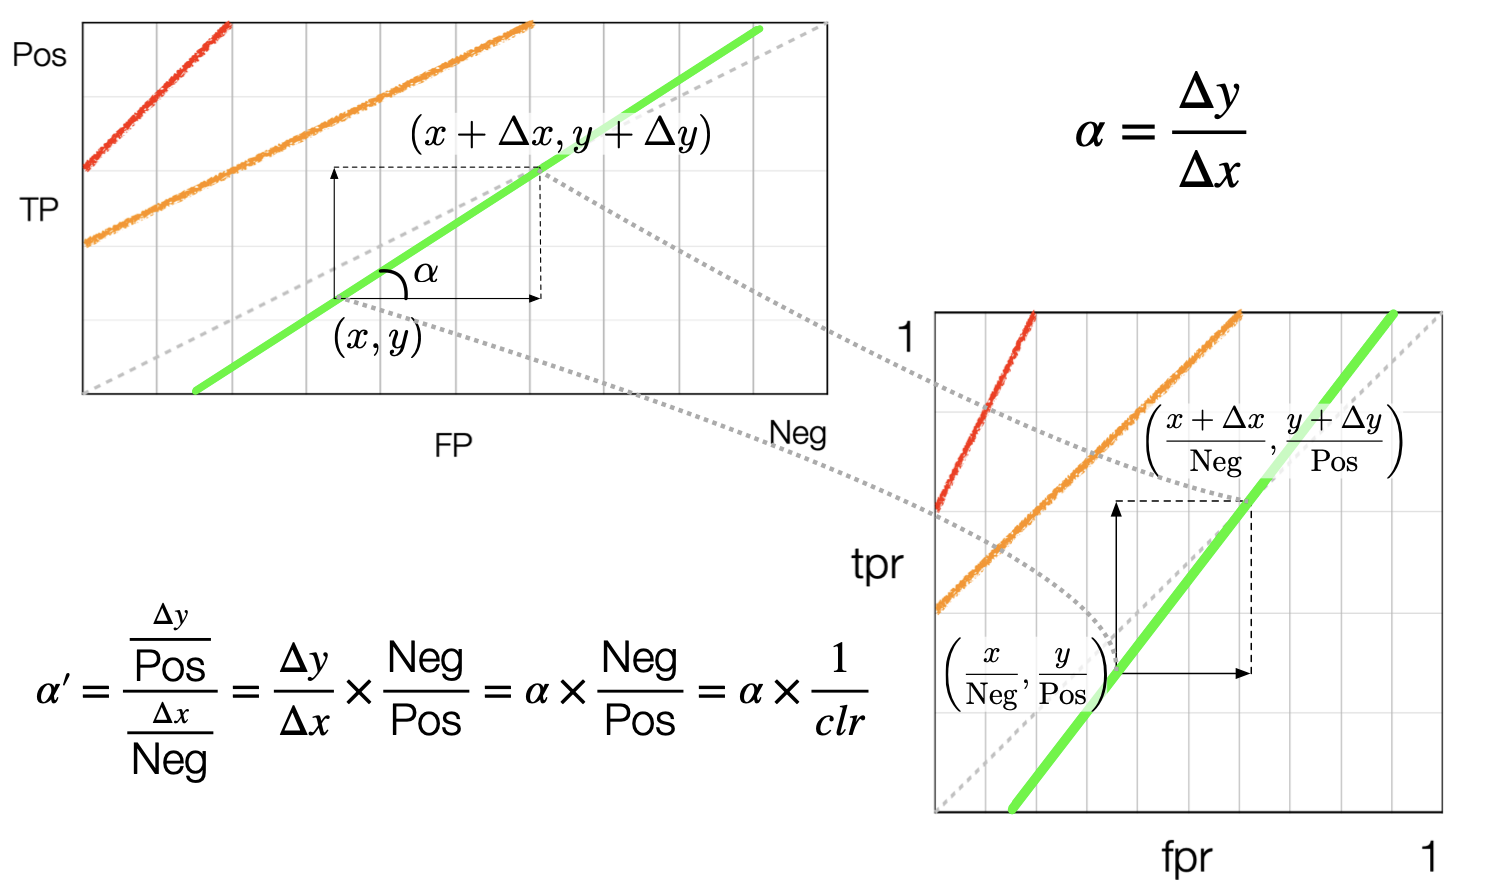
\includegraphics[scale=0.5]{images/rocPlot.png}
    \label{fig:enter-label}
\end{figure}

Quindi l'\textbf{accuratezza} cambia, i classificatori che stanno su rette con pendenza $\alpha = \frac{Neg}{Pos}$ hanno la stessa accuratezza. Punti che stanno su rette con pendenza 1 hanno la stessa \textbf{average recall}. 

\paragraph{Da un singolo decision tree derivano molti classificatori.}
\begin{figure}[!h]
    \centering
    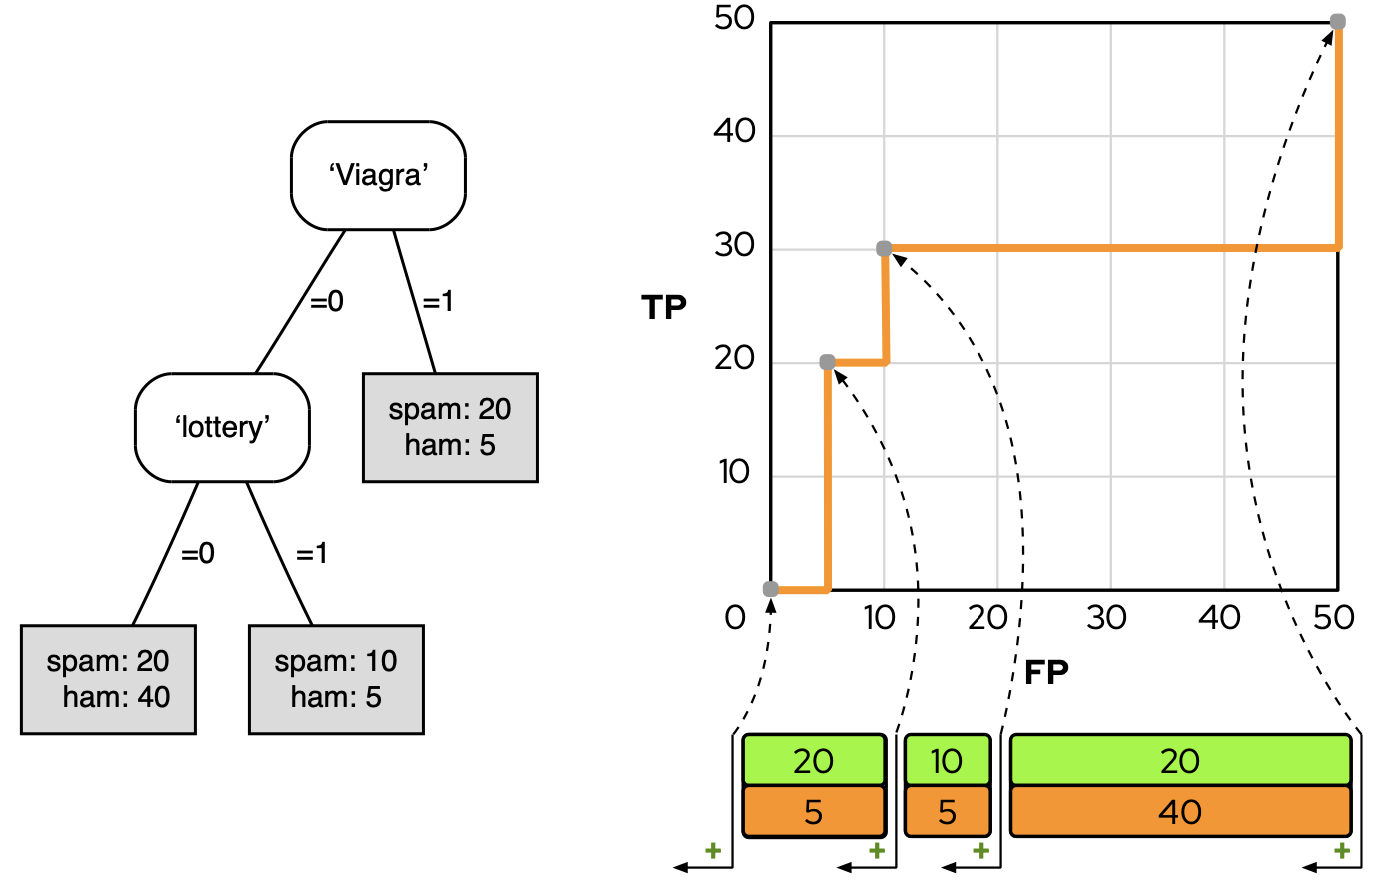
\includegraphics[scale=0.5]{images/decTreeClass.png}
    \label{fig:enter-label}
\end{figure}
Scegliamo una \textbf{treshold} e decidiamo che tutto ciò che è alla sua sinistra è considerato negativo e tutto cioò che è alla sua destra è considerato positivo. Nel momento in cui scegliamo una nuova treshold stiamo creando un nuovo classificatore. Per esempio, se scegliamo come treshold 10 sull'asse delle x, la prima foglia è considerata positiva, le altre no (arancioni=negativi, verdi=positivi). I falsi positivi saranno 5 e i veri negativi saranno 20.

\newpage

In verità, a \textbf{seconda di come assegnamo i costi ai FP e FN, la risposta alla domanda "qual è il classificatore migliore?", cambia}. Assumendo un costo $FP=FN$, allora il punto (10,30) è il migliore. Ma se scelgo un costo $FP=2FN$ allora (10,30) e (5,20) sono sulla stessa isometrica e posso scegliere indifferentemente uno dei due. Se il costo $FP=4FN$, il punto che sovrasta tutti sarebbe (5,20).
\begin{figure}[!h]
    \centering
    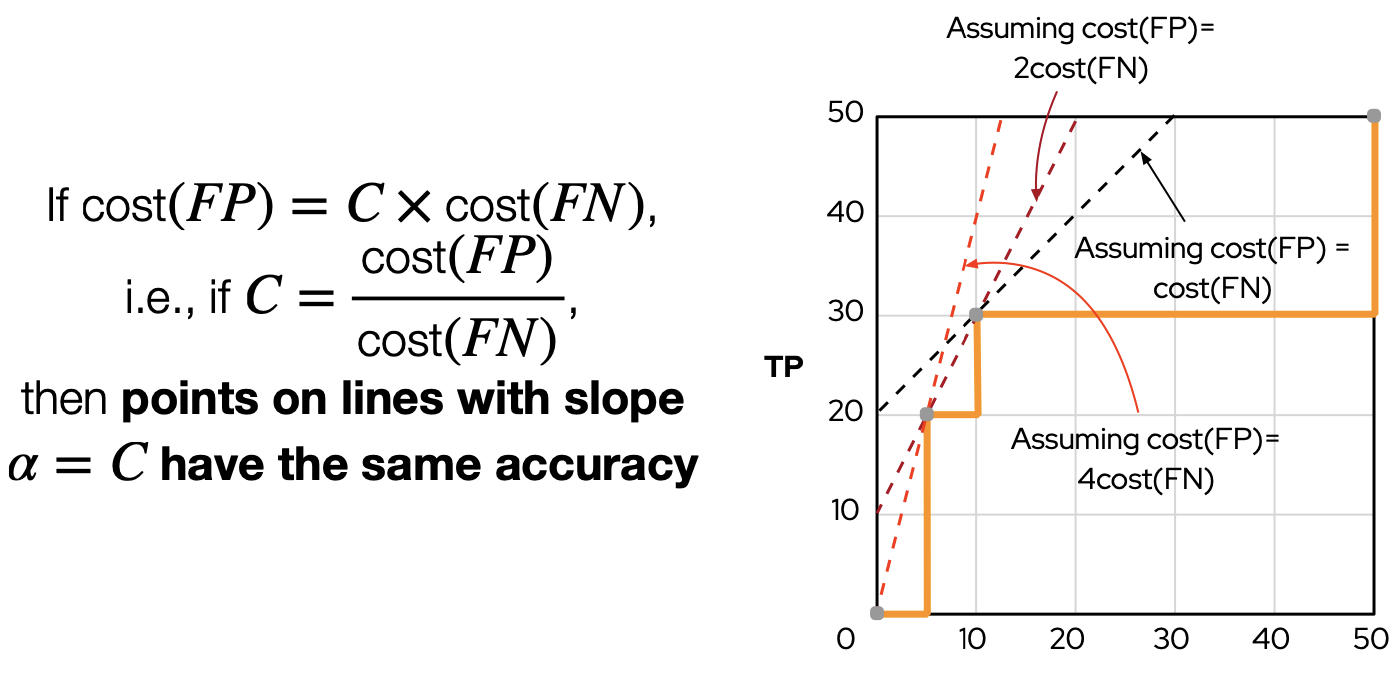
\includegraphics[scale=0.5]{images/changeCost.png}
    \label{fig:enter-label}
\end{figure}

Quindi se C è il rapporto tra i costi, \textbf{i punti sulle rette con pendenza $\alpha$ hanno la stessa accuratezza}.

\paragraph{Ma perchè questo è vero?} Innanzitutto dobbiamo ridefinire la misura di accuratezza.
\begin{equation}
\begin{split}
    x=FP    \\
    y=TP    \\
    acc=\frac{TP+TN}{TOT}=\frac{TP+TN}{Pos+Neg}
\end{split}
\end{equation}
Ricoridamo che, dalla tavola di contingenza $TN=Neg-FP$, quindi
\begin{equation}
    acc=\frac{TP+Neg-FP}{Pos+Neg}
\end{equation}
Ma cosa vuol dire che il \textbf{costo dei positivi è C volte il costo dei negativi?} \'{E} come immaginare di avere un nuovo dataset in cui tutti gli esempi negativi sono replicati 4 volte. In questo modo, ogni volta che faccio un errore su un negativo, sto facendo 4 errori. Da qui:
\begin{figure}[!h]
    \centering
    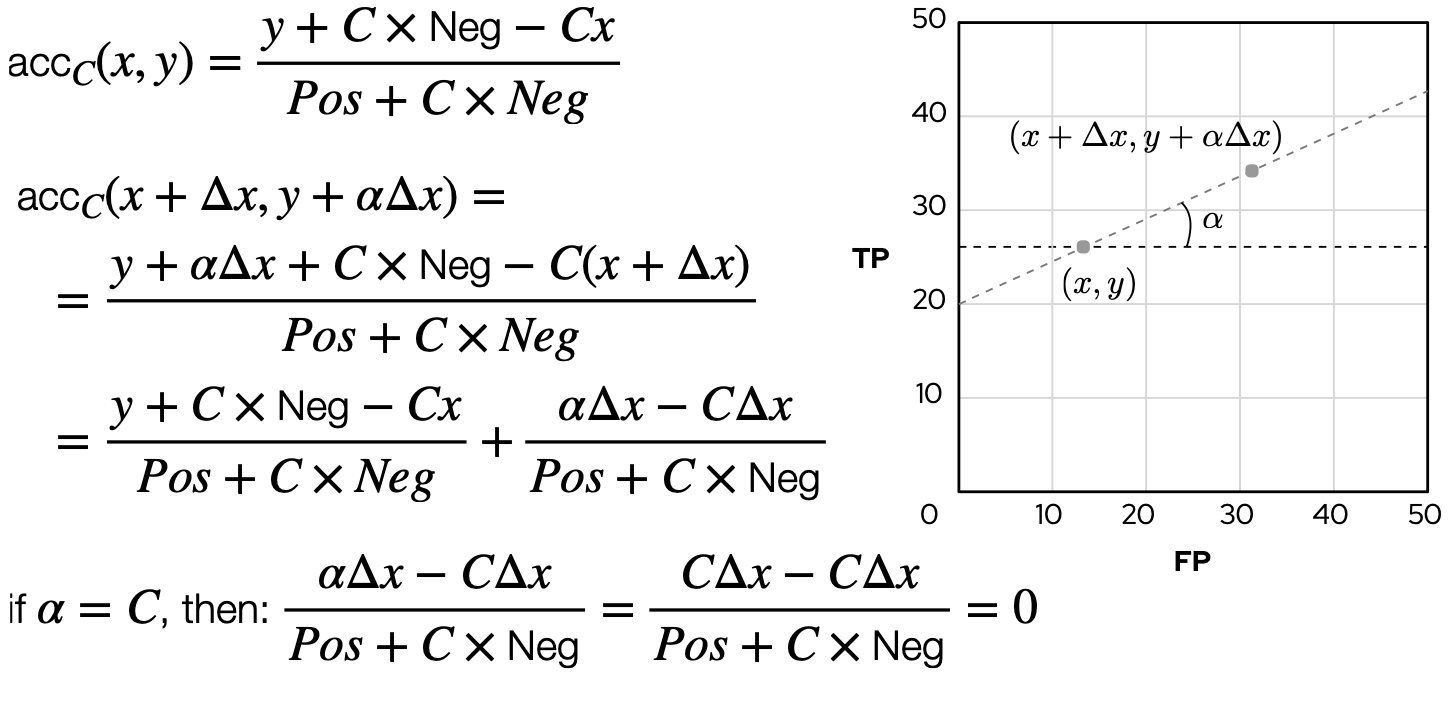
\includegraphics[scale=0.5]{images/newAcc.png}
    \label{fig:enter-label}
\end{figure}

Nei \textbf{ROC plot}, per ottenere la stessa isometria, moltiplico per $\frac{1}{clr}$ dove $clr=\frac{Pos}{Neg}$.
